%\documentclass[10pt]{revtex4-1}
\documentclass[10pt]{article}
\listfiles               %  print all files needed to compile this document
\usepackage{blindtext}

\usepackage{amsmath}
\usepackage{xparse}
\usepackage{graphicx}
\usepackage{dcolumn}
\usepackage{bm}
\usepackage[colorlinks=true,urlcolor=blue,citecolor=blue]{hyperref}
\usepackage{color}
\usepackage{physics}
\usepackage{algorithm2e}
\usepackage{algpseudocode}
\usepackage{pgfplots}
\usepackage{pgfplotstable, booktabs, mathpazo}
\usepackage{natbib}

\pgfplotsset{compat=1.15}

\pgfplotstableset{
    every head row/.style={before row=\toprule \hline ,after row=\hline\hline \midrule},
    every last row/.style={after row=\hline \bottomrule},
    every first column/.style={
        column type/.add={|}{}
        },
    every last column/.style={
        column type/.add={}{|}
        },
}
\pgfplotstableset{
    every head row/.style={before row=\toprule \hline ,after row=\hline\hline \midrule},
    every last row/.style={after row=\hline \bottomrule}
}

%\begin{figure}[hbtp]
%\includegraphics[scale=0.4]{.pdf}
%\caption{}
%\label{fig:}
%\end{figure}

%\begin{tikzpicture}
%    \begin{axis}[
%            title= Earth-Sun system, Forward Euler integration,
%            xlabel={$x$},
%            ylabel={$y$},
%        ]
%        \addplot table {../runresults/earthEuler2body.dat}
%    \end{axis}
%\end{tikzpicture}

\title{Project 3
	Wisconsin Cancer data and Logistic regression and Feed Forward Neural Networks}
\author{Annika Eriksen}

\begin{document}

\maketitle

\begin{abstract}
	The wisconsin cancer data is a staple of machine learning and should therefore 
	be a good point to analyse different methods. I analyze the data using 2 different 
	methods, firstly through logistic regression and later on using a Feed Forward Neural
	Network 
\end{abstract}

\section{introduction}

The Wisconsin Cancer dataset is a widely used set for classification
problems, and offers a good starting point to compare implementations of
machine learning methods. I have put the set through 2 different methods,
Logistic regression and a Feed Forward Neural Network. 

First, the Logistic regression takes in the data and feeds it into the
sklearn logistic regression method.  This is done without- and then with
scaling the data to see prediction accuracy depending on these. Then I take
only those features with the greatest correlation to a malignant tumour and
train the set on those only, to see the predictive ability of the methods
based on these. 

While we see an expected increase in accuracy after normalising the features,
there is a rather unexpected decrease in accuracy when only including the more
important features.

Then, Implementing a Feed Forward Neural Network (ffnn), We construct a
network with 1 hidden layer and a binary input, either malignant or benign.
The initial model is then iterated a number of times, or until the
predictive accuracy of the model on the test set has passed it's peak. 

As one expects, the neural net quickly goes toward an above 90\% accuracy for
both training and test set until eventually overfitting sets in and the test
set accuracy starts to fall off. 


%\section{theory}

\section{methods}

%insert the theory for logistic regression and ffnn, see lect. notes and the
%relevant course literature mentioned there. 

\subsection{Logistic Regression}
The base problem to be solved with the cancer data set is a binary benign vs.
malignant tumor, 0 or 1 encoded respectively, 

\begin{align}
y = 
	\begin{bmatrix}
		0 & \text{benign} \\
		1 & \text{malignant}
	\end{bmatrix}.
	\label{yclass}
\end{align}

We have 2 \emph{classes}, which form the entirety of the possible outcomes within
the set. Like with regression I want a model to give an expected value for a given 
set of samples for the features. A way to model would be to assume some linear functional
dependence, along the lines of

\begin{align*}
	f(y_i|x_i) = \beta_0 + \beta_1 x_1.
\end{align*}

Although this could contain values outside of 0 and 1. Taking the mean solves
this and forces $f(x|y) \in [0, 1]$. This then can be seen as the probability
for finding a given value for $y_i$ with a given $x_i$. This S-shaped function
would give us the \emph{sigmoid} function. 	
%TODO note that the perceptron model deals with a hard predictor, as opposed to
%the soft predictor of logistic regression.
The soft predictor gives a probabilistic prediction of the class of outcome,
given the input feature. In my case, this is either of the options in
y in eq \ref{yclass}.  The Sigmoid, or \emph{logit} function governs this
probability prediction for a given event thus,

\begin{align}
	p(t) = \frac{1}{1 + \exp(-t)} = \frac{\exp(t)}{1+\exp(t)}
	\label{logit}.
\end{align}
Noting, $1 - p(t) = p(-t)$.

Since we have 2 possible outcomes, the probabilites are then given by
\begin{align}
	p(y=1|x_i, \hat{\beta}) &= \frac{ \exp(\beta_0 + \beta_1x_i) }
								{ 1 + \exp(\beta_0 + \beta_1x_i) } 
								\label{prob1}\\
	p(y=0|x_i, \hat{\beta}) &= 1 - p(y=1|x_i, \hat{\beta})\label{prob0}.
\end{align}
Denoting the biases with $\mathbf{\beta}$ which I want to extract from the dataset. 

Using the Maximum Likelihood Estimation %TODO cite from Hastie or Geron
principle The total probability for all possible outcomes of a dataset
$\mathcal{D} = {(y_, \mathbf{x_i)}}$, with the binary in eq. \ref{yclass} for
each $y_i$. The probabilities can be approximated by a product of the
individual probabilities for an outcome of $y_i$,

\begin{align}
	\mathbf{P}(\mathcal{D}|\hat{\beta}) 
		= \prod_{i=1}^n\qty[p(y_i=1|\hat{\beta})]^{y_i}
			\qty[ 1 - p(y_i=1|\hat{\beta}) ]^{1-y_i}
\end{align}
And from this we can find the log-likelihood and our \emph{loss} function. 
\begin{align}
	\mathcal{C}(\hat{\beta}) = 
		\sum_{i=1}^n \bigg( 
			y_i \log\big[p(y_i=1|x_i\hat{\beta})\big] + 
			(1 - y_i)\log\big[ 1 - p(y_i=1|x_i\hat{\beta})\big]\bigg).
\end{align}

Inserting for the probabilities with eq. \ref{prob1} and sorting the logarithms, we can
rewrite the loss function. The cost/error function is the negative log-likelihood function, so it
would be the negative of this rewrite. The end result then, is

\begin{align}
	\mathcal{C}(\hat{\beta}) = 
		-\sum_{i=1}^n \qty(y_i(\beta_0 + \beta_1x_i) - \log(1 + \exp(\beta_0 + \beta_1x_i)))
		\label{costfunc}.
\end{align}
This is also known as the cross-entropy. This can be further supplemented with regularization
parameters much like with Lasso and Ridge regression. 

The next step then is to minimize the cost function. Differentiating wrt. $\beta_0$ and $\beta_1$
and compacting, gives us

\begin{align}
	\pdv{\mathcal{C}(\hat{\beta})}{\hat{\beta}} = 
		- \mathbf{\hat{X}}^T (\hat{y} - \hat{p}).
	\label{Cost1stDerivative}
\end{align}

Where $\hat{y}$ is a vector with the values $y_i$, $\mathbf{\hat{X}}$ is an
$n\times p$ matrix containing the $x_i$ values. The vector $\hat{p}$ contains
the fitted probabilities $p(y_i|x_i,\hat{\beta})$. For a step further and
introducing another matrix, $\mathbf{\hat{W}}$ with elements
$p(y_i|x_i,\hat{\beta})(1 - p(y_i|x_i,\hat{\beta})$, we can arrive at a more
compact version of the 2. derivative. 

\begin{align}
	\pdv[2]{\mathcal{C}(\hat{\beta})}{\hat{\beta}}{\hat{\beta}^T} 
		= \mathbf{\hat{X}}^T \mathbf{\hat{W}} \mathbf{\hat{X}}
	\label{Cost2ndDerivative}.
\end{align}

With the regression model accounted for, the script itself imports and uses the
\emph{scikitlearn} module in python, where the data is loaded from, scaled and
split into training and testing sets in various permutations. The regression itself is
mainly done with scikitlearn's \emph{LogisticRegression} method, implementing
the mathematics above with a well documented and tested code. It is also
optimized well beyond the possible approach of this project. It is therefore an
easy to use tool to check the data. 

Once the data set is loaded and some parts are displayed, 3 different
regressions are made. 1 for the raw set, one where the feature data is scaled
and one where a percentage of the most important features are selected for and
trained on.

\subsection{Feed Forward Neural Net}

A neural network is a computational model which aims to imitate the workings of
biological neurons, where an arbitrary amount of layers, each with an arbitrary
number of neurons exchange signals in the form of mathematical functions. These
systems take in example inputs and configures an output without any specific
rules for a given task

The basic idea is that each neuron collects incoming signals. If the signals exceed
a given activation threshold, the neuron fires as well. the signals failing to meet this
threshold leave the neuron inert and there is no signal. A simple mathematical model of this
can be written,

\begin{align}
	\mathbf{y} = \mathbf{f}\qty(\sum_{i=1}^n \omega_i x_i) = \mathbf{f}(\mathbf{u})
	\label{simpleNeuron}. 
\end{align}

Where the output $y$ is the output of the activation function and takes the
input of a weighted sum of n other neurons. Though there are various types,
e.g. Convolutional neural networks for image recognition, The focus for this
will be a simple general purpose one for supervised learning, seeing as the
cancer data is already properly labeled. 

The model used in this project is a Feed forward Neural network. This is the
first type developed and the simplest type. Here, the information flows only
one way. Each node in a layer is connected to every other node in the next
layer, mediated with weights. Therefore called a \emph{Fully Connected FFNN}

A neural net with 3 or more layers, an input and output layer with one or more
hidden layers between, is frequently called a \emph{Multilayer Perceptron
(MLP)}. These are utilized because the \emph{universal approximation theorem}
shows us that Given a non-constant, bounded and monotonically increasing
activation function for the hidden layer.  Given a non-constant, bounded and
monotonically increasing activation, an MLP can predict a continuous
multidimensional function to arbitrary accuracy with only 1 hidden layer and a
finite set of neurons.

The output is then given by the function 

\begin{align}
	y = f\qty(\sum_{i=1}^n(w_ix_i + b_i)) = f(z)
	\label{eq:activationFunc}.
\end{align}

This is similar to equation \ref{simpleNeuron}, but with an added intercept per
node. The MLP is fully connected, as stated above. Thus each node receives a
weighted sum of the output of every other node in the previous layer. 

For the first hidden layer, each node $z^1_i$ is then a weighted sum of the
outputs of the nodes int the input layer. 

\begin{align}
	z^1_i = \sum_{j=1}^N w^1_{ij}x_j + b_i^1
	\label{eq:nodeInput}.
\end{align}

The $b^1_i$ is the bias for the node, which is needed in the case of a 0 input.
The value of this sum is the input into the activation function, eq.
\ref{eq:activationFunc}, for the i-th node. The summation is over all $N$
possible inputs into the first layer.

More generally, we can assume that the nodes within a layer share an activation function
but that the activation functions could vary between layers. This can be shown with a superscript
$l$.

\begin{align}
	y^l_i = f(z^l_i) = f\qty(\sum_{j=1}^{N_{l-1}}( w^l_{ij}x^l_i ) + b^l_i ).
\end{align}

Here, the $N_{l-1}$ denotes the number of nodes on the previous layer, as the
$M$ in equation \ref{eq:nodeInput} denotes the number of nodes in the input
layer. This process can be repeated through the layers, Feeding Forward to the
output layer. This expression eventually becomes then a sum of the sum of the
sums of the previous layers. In essence, then the only independent variables in
the system is the initial values. The rest inductively follow. 

With the input settled, the question of activation function comes next. As
mentioned wrt. the universal approximation theorem , the activation function
has a few requirements. The activation function must be non-constant, bounded,
monotonically-increasing and continuous. The second option here excludes any
linear function. In order to avoid the neural net producing a linear
transformation through the layers, some non-linearity is needed. A common
activation function is the \emph{sigmoid function}

\begin{align}
	f(x) = \frac{1}{1 + \exp(-x)}
	\label{eq:sigmoid}
\end{align}

There are many other options, but they are not explored with this project.
There are some issues with the sigmoid function wrt. gradient descent methods
as the gradients can tend to disappear for the sigmoid, despite it's initial
popularity due to the similarity with the potential curves within the
biological neurons. A more popular function is the $\tanh$ function. 

With the layers and nodes described as well as the signal connecting them from
input to output, There remains an issue of predictive ability. Sending the data
through and setting the weights the once is not the best basis for such things.
To improve the results, we can adjust the weights once we've found an output.
The method for this is the \emph{back propagation algorithm}

The back propagation error is
\begin{align}
	\delta^l_j = \sum_k \;\;\;\delta^{l+1}_k \;\; w^{l+1}_{kj} \;\; f'(z^l_j)
\end{align}

Which we apply once the layers have been passed through forward, using the
outputs of each layer and propagating the errors backwards. Using gradient
descent, we update the weights of each node according to the gradient and the
learningrate. 

%TODO describe neural nets

\section{results}

The results for the Logisti regression case provides a good approximation of
the data, where the naive implementation on the data without scaling it
predicts with an accuracy of 96\%. Scaling the data provides a better
predictive accuracy by culling outlying data, bringing the accuracy of the
model up to 98\%.  Finally with the regression case, removing the less
important data and training only on those provides a poorer predictive accuracy
than the 2 sister methods at 95\%, see table \ref{tab:logreg}

\begin{table}
	\centering
	\begin{tabular}{ |c|c| }
		\hline
		Full set, unscaled & 0.96 \\
		\hline
		Full set, scaled & 0.98 \\
		\hline
		exclusive features, scaled & 0.95 \\
		\hline
	\end{tabular}
	\caption{Logistic regression scores for Wisconsin Cancer data. The unscaled
	data provides a predictive accuracy of above 95\%, with the scaled data
	gets as far as 98\%. The final selection uses only those features of the
	data that have the best correlation with a malignant and benign tumor.
	Here the accuracy score drops }
	\label{tab:logreg}
\end{table}

For the neural network the accuracy of the prediction quickly climbs to 94\% accuracy for both the 
training and test set after fewer than 10 epochs. Then the growth mellows somewhat. The training
accuracy grows to about 99\% and remains stable here, the test accuracy climbs to a maximum of 97\%
after 200 epochs. The test accuracy eventually begins to taper off again towards the end. After roughly
600 epochs, the system is as accurate at predicting other data as it can be. Continued training at this
point, as the predictive accuracy falters. The 2 accuracies can be seen in figure \ref{fig:ffnnaccuracy}

\begin{figure}[hbtp]
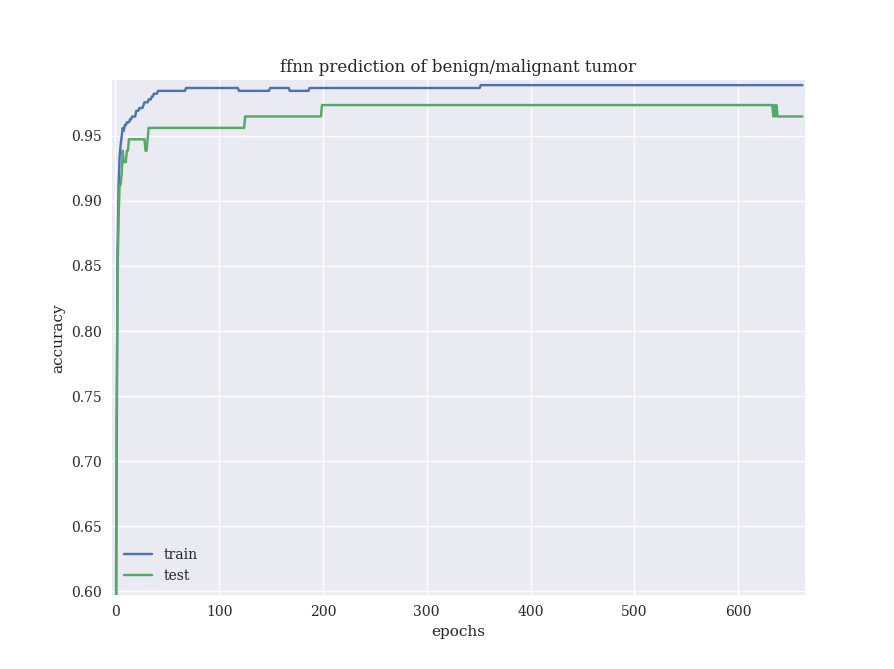
\includegraphics[scale=.6]{../ffnnaccuracy.png}
\caption{Plot of the accuracy of prediction of the neural net for the Wisconsin
	cancer data set.  The accuracy is the ratio of accurate predictions over
	the different epochs. The blue training accuracy quickly goes to ~0.99,
	while the test sett accuracy peaks some 150 epochs later at ~0.97 before
	lowering gradually after about 600 epochs.}
\label{fig:ffnnaccuracy}
\end{figure}

% Here go the results of the tests, the display of the data (unless implemented in methods)
% here goes the prediction results and the accuracy plots. 
% Also discuss, though do no conclude the results. 

\section{conclusion}

The results from the logistic regression points towards predicting based on all features rather than 
stripping away the less relevant features. This seems counterintuitive. A more likely outcome is an 
error in either the selection of relevant features, based on the correlation between the feature in 
question and the output values, or in the implementation of the scoring values. 

% Here we wrap up the analysis and actually discuss and draw conclusions. 
% Also pull in other works and wonder on future improvements and further work
\blindtext

%\section{appendix}

%The appendix would be for any maths, tables or graphs that don't quite fit into the
%body of the text. Also a potential place for code, though I imagine I will merely refer to
%github for this. 

%\bibliography{\string~/Documents/bibliography/Bibliography}

\end{document}

